\documentclass[format=acmsmall, review=false, screen=true, anonymous=True]{acmart}
\usepackage{graphicx}

\begin{document}

\title{Agile Software Development}
\author{Arizona State University, SER 515}



\begin{abstract}
Software engineering, despite sharing the nomenclature of "engineering", suffers from vastly different design, development, and release problems than the so-called "traditional" engineering fields (mechanical, civil, aeronautical, etc.). Initial requirements gathering is more complicated and psychological (it is often said that "the end user does not even know what they want") and the systems themselves can quickly become impossible for a single individual to comprehend in its entirety. Agile software development hopes to address and improvement upon the failure of the classical engineering model.
\end{abstract}

\keywords{Agile stakeholder developer engineer iteration}

\maketitle

\section{Introduction}
Agile is a software development methodology that attempts to address the issues of rigid, "no turning back", development as well as low end user feedback cycles. In the past, software engineering merely borrowed its methodologies from sister engineering disciplines. This proved to be disastrous for many and was, unfortunately, not immediately recognized as disastrous to the practitioners and managers of the early software development projects. Engineering was handled in a traditional, "measure twice, cut once", fashion. That is, a project could spend years, if not more, simply designing and planning before any implementation was attempted. By the time the project was finally completed the end user had moved on, either to another technology. Or they simply did not need the product anymore. Or perhaps the initial requirements given by the customer were flawed, and now years of design of development has gone towards incorrect specifications. Or worse yet, once development had finally started, the design had hidden within it flawed basic assumptions, rendering the whole thing useless.

In Agile, rather than a pipeline approach to development, an iterative approach is adopted instead. Smaller chunks of the product are designed, developed, demonstrated and refined. These smaller features are introduced to the end user more frequently, allowing for a more rapid feedback loop and thus faster error correction with regard to requirements specification. For the end user, they see the benefit of constant progress updates as well as the empowerment of providing useful, immediate, feedback.
\section{Agile}
Agile, as a philosophy, is about satisfying the core desires from two disparate, yet intimately interacting, groups - the stakeholders and the developers. The stakeholders are, for example, end users, management, investors, operations and so on. That is, stakeholders are the people who have an acute interest in the software, either because they want to use it or they want to make money off of it. However, they are not the ones actually creating the software. The ones creating the software are the developers. These developers can be broken up into broad roles, such as leads, owners, and rank-and-file engineers.

\begin{figure}
  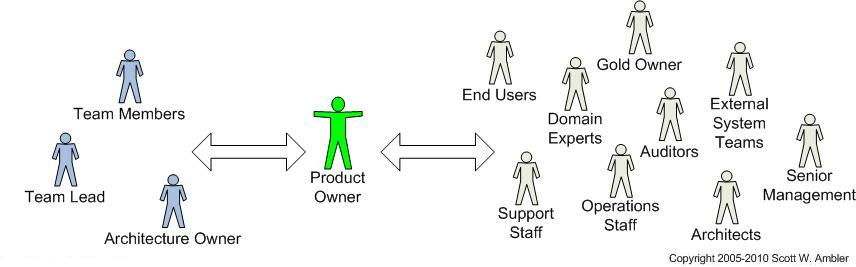
\includegraphics[width=\linewidth]{productOwner.jpg}
  \caption{Fig 1. Product owner represent a range of stakeholders (Scott W. Ambler, 2012).}
\end{figure}

\subsection{Developers}
Core to the benefit that the developers experience from the Agile process is the practice of iteration. In traditional manufacturing or engineering, the acts of design, execution, testing, and shipment all occur in a pipeline. That is, once design is done then the product is built. Once the product is built, then it is tested. Once it has passed all testing, then it is finally shipped. All stages must be completed in its entirety before moving on to the next phase of the pipeline - going back up the pipeline is very rare, if not impossible. This traditional engineering practice is called Waterfall (the very name seems to convey this "one-way-only" approach, after all you cannot swim back up a waterfall). Unfortunately, despite the seemingly close resemblance to traditional engineering, Waterfall has proven disastrous in the practice of software engineering. A lack of knowledge about what the actual requirements are can lead under/overdevelopment, redevelopment, and generally a massive loss in revenue due to increased costs [2].

Combating Waterfall’s disastrous approach with a proper feedback and refinement loop is at the heart of Agile’s value proposition for developers. It may be helpful to look at the iteration of a product development more formally. Let an end product of a software project be called $P$. Let $Q$ be a function of some arbitrary quality, such that if $Q(P)$ holds true then $P$ is said to be of "high quality". In Waterfall, the goal is start with nothing and then to one day arrive to $Q(P)$. However, in Agile, rather than $P$ being put through design, execution, testing and shipment as a whole, $P$ is broken into many smaller, atomic features $\{F\textsubscript{1}, F\textsubscript{2}, F\textsubscript{3} ... F\textsubscript{n}\}$. With all components completed and integrated it can be said that $P = \{F\textsubscript{1}, F\textsubscript{2}, F\textsubscript{3} ... F\textsubscript{n}\}$. Agile says that $\{\forall F \in P | Q(F)\}$. That is, every feature in $P$ must undergo its own design, construction and quality assurance cycle. If a feature does not satisfy $Q(F)$ then it re-enters development in an iterative fashion. That is, rather than the product as a whole going through a single, all-or-nothing, pass at quality assurance each feature actually gets a development cycle all to itself. At the end of each cycle the feature is demonstrated to the stakeholders and the quality of the feature is determined. The stakeholders may approve of the quality of the feature or they may provide feedback as to why it does not meet their standards. Either way, each feature receives feedback from the stakeholders, thus ensuring that the developers are continuously addressing the needs and wants of the stakeholders rather than dumping an entire product onto them which may or may not be changeable in the future. Every cycle of iteration must result in a working product of some kind with minimal bugs [3]. This process provides value to the stakeholders as well as saving a world of pain for developers who might otherwise build features that are completely inappropriate and difficult to modify.

\subsection{Stakeholders}
The stakeholders have the luxury, as well as the burden, of receiving and providing near constant feedback.

  From a managerial point of view Agile has proven to be wildly attractive for the purposes of progress tracking. That is, development has been granularized to such a degree that accurately charting, and thus guiding and predicting, a project becomes far more accurate and easier to do. Since features are developed one at a time, developers can also be made to be more myopic and thus more easily corralled from week-to-week.

  From an end user point-of-view a frequent progress update is incredibly comforting. First is the mere access to greater, and more frequent, information about the product that they are buying. The end user may have their own development cycles and customer requirements that, in turn, are dependent upon your output. The ability to not only see the incremental results, but to help guide the results to their own specification, is empowering for the end users.

\section{Conclusion}
Agile has gone a long way to address the failures of older, classical, engineering practices. It reigns as the most popular methodology in the industry as of writing this, and can be found in almost (if not all) of the major Silicon Valley firms, and these are some of the largest, most visible, projects on the planet. It has even reached out into popular culture as the television show Silicon Valley had parodied a development team’s "burn down chart" (a graph measuring progress often used in Agile). Indeed, Agile has had a strong track record of success over the past decade, if not longer. Its iteration over the product is well liked by developers since it gives a nod to the difficulty of the task. Meanwhile, the constant feedback is appreciated by stakeholders that those stakeholders who may be the end users may even call it a feature of the product (if only they were more aware of Agile and its uses). Even if Agile itself does not withstand the longer test of time, its iterative approach will likely be appropriate by future generations since it has proven so useful.

\section*{References}
[1]  Scott W. Ambler. (2005-2012). "Roles on Agile Teams: From Small to Large Teams".
 Retrieved August 26, 2017 from http://www.ambysoft.com/essays/agileRoles.html.

\noindent[2] Parnas, David L.; Clements, Paul C. (1986). "A rational design process: How and why to fake it". Software Engineering, IEEE Transactions: 251–257. Retrieved September 2, 2017 http://www.cs.tufts.edu/~nr/cs257/archive/david-parnas/fake-it.pdf.

\noindent[3] Beck, Kent (1999). "Embracing Change with Extreme Programming". Computer. 32 (10): 70–77. Retrieved August 25, 2017 from http://ieeexplore.ieee.org/document/796139/.

\end{document}
